A crowdsourcing video annotation process in which four different microtasks were cascaded was developped to evaluate the proposed approach. In the process, extra content such as images, text, hyperlinks and other elements are applied in the video enrichment. The computational support to the experiment was supported by a toolkit that includes all annotation tools and aggregation methods required to perform the microtasks. Moreover, the presentation system capable to play the enriched videos was also provided.

The presentation system play coherently the video and the extra content produced and positioned by the crowd, according to the annotations provided by them.

All the tasks performed by the workers were designed to be simple, easy and small, and through them everything was done by the crowd: interesting points identification, content providing, content ranking, even to determine the position at which each content should be displayed on video scenes.

The crowd involved in this experiment was recruited by an open call that consisted of a broadcast message posted on a social network, asking volunteers to access an annotation tool and use it to contribute to an academic work. Of course, the reach of the open call would be much greater, also the number of contributions, if a commercial system such as Amazon Mechanical Turk or CrowdFlower was used, but it would require financial resources that were not available \cite{Difallah:2015:DMC:2736277.2741685}. However, the open call worked fine and the number of contributions received was sufficient to generate the desired outcome.

Each microtask has been activated for 24 hours, then it was closed and the specific aggregation method was executed. After the aggregation method produced the result for a microtask, the next one became active, taking that result as input. To take advantage of the first open calls, the strategy was to use the same URL for all microtasks, redirecting the contributor to the microtasking that was currently active.

The decision to leave each microtesk active for 24 hours had two reasons: to share the time available for the experiment among all microtasks in a balanced way and to measure how many contributions can be acquired by a subtle open call in a single day. 

In order to reduce duplicate contributions without the need to register contributors, it was collected a fingerprint using the IP address and Web browser ID for each contribution \cite{mulazzani2013fast,segundo2016crowdsourcing}. This technique provided a good indication of who was contributing, so it was possible to discard multiple contributions from the same brand for the same item to be annotated. As tasks 1 and 2 aimed to collect as many items as possible from the crowd, this technique was applied only in tasks 3 and 4, in which workers contributed based on the items already registered in the system. However, even in tasks 3 and 4 the system accepted annotations with the same fingerprint for different items.

In this experiment, two annotated videos with approximately 1 minute duration were produced using the cascade process. Next, this experiment is detailed showing the steps defined in the proposed approach.

\subsection{Step 1: Preparation}
Before beginning this step, it is important to determine which kind of annotations should be generated at the end of the process. In this case, the annotated video must be related to items displayed at certain positions in specific scenes. This way, the following features must be specified:
\begin{itemize}
\item \textbf{Determine which objects must be annotated:} \linebreak  
The items to be observed in these experiments are called Points of Interest. Each point of interest is related to one of these types of occurrences.
\begin{enumerate}
\item Expression that requires synonyms or definitions; 
\item Information that requires additional explanation.
\end{enumerate}

\item \textbf{Determine attributes to be annotated on each object:} \linebreak  
Each point of interest must be annotated in two aspects.
\begin{enumerate}
\item Which content should be displayed over it;
\item In what position the content should be displayed.
\end{enumerate}


\item \textbf{Describe a microtask for each pair object-attribute:} \linebreak  
To achieve the desired annotated video, a microtask is needed to identify the points of interest, two microtasks to collect their attributes and a microtask to ranking the suggested content to be associated with each point of interest.

\begin{itemize}
\item \textbf{Task 1: Identify the points of interest.} Workers should watch video segments and mark a point of interest if found, and identify its subject using plain text. This text can be a word or a phrase according the point of interest.

\item \textbf{Task 2: Suggesting contributions content.} Workers receive a random point of interest and suggest some content to cover it. The provided content may be an image, a hyperlink to a website, or plain text.	

\item \textbf{Task 3: Ranking the provided contents.} Workers receive a random suggested content for a point of interest and vote on the most appropriate.
	
\item \textbf{Task 4: Positioning the items over a scene.} 
Workers receive a random scene associated with a point of interest, and an item that should be positioned over the scene in order to reduce occlusion problems. In this task, each position is captured as a coordinate pair [X,Y] considering the superior-left corner of the video as the coordinate [0,0].

\end{itemize}

\item \textbf{Define an aggregating method for each microtask:} \linebreak  
According to the approach followed, it is necessary to define an appropriate aggregation method for each microtask.

\begin{itemize}
\item \textbf{Task 1: Temporal grouping.} Identified points of interest are grouped by time, with a tolerance of 0.5 seconds. For each group, a content analysis is performed to merge equivalent contributions. Finally, the predominant input is selected and marked as the point of interest at that time in relation to the timeline.

\item \textbf{Task 2: Grouping by point of interest.} The content provided by contributors in task 2 is grouped by point of interest. Therefore, a content analysis is done to bring together equivalent contributions.

\item \textbf{Task 3: Ranking by voting.} For each point of interest, the most popular suggestion is selected based on contributions to task 3.
	
\item \textbf{Task 4: Average coordinates.} The contributions are grouped by point of interest and, for each point, the average coordinate is determined.

\end{itemize}


\item \textbf{Build a simple annotation tool for each microtask:} \linebreak 
Still following the presented approach, a simple annotation tool must be built for each microtask. Each of these tools is designed to collect a specific annotation.

%To improve the user experience the user interfaces of all tools were designed to be visually similar, with the contribution form always located on the right.

%, the video player is always located on the left, the contribution form on the right, and the instructions are always located at the top of the page.

\begin{itemize}
\item \textbf{Task 1:} The first annotation tool (Figure~\ref{task1}) consists of a video player, with a navigation bar that allows the collaborator to watch the video and pause it at the moment the point of interest is found. Thus, the worker can write the subject for this and send the contribution.
\begin{figure}[h]
	\centerline{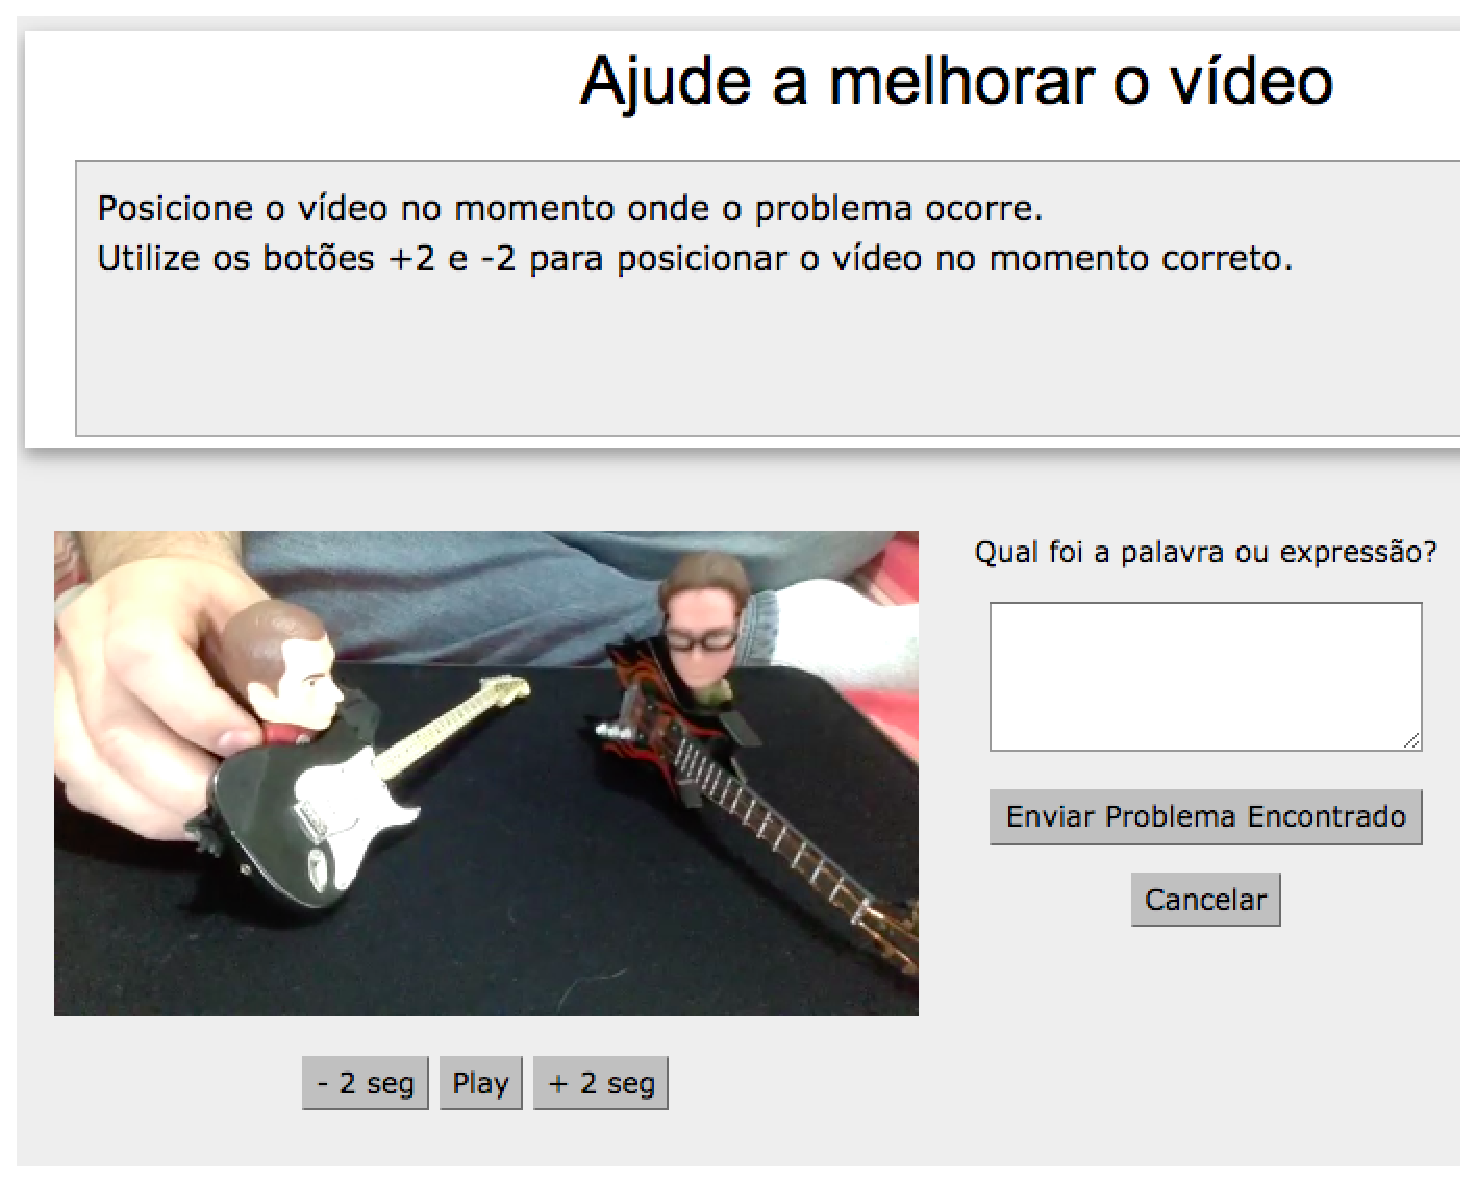
\includegraphics[scale=0.28] {figure/task1_c}}
	\caption{Annotation tool for task 1}
	\label{task1}
\end{figure}  

\item \textbf{Task 2:} the second annotation tool (Figure~\ref{task2}) presents the collaborator a point of interest and positions the video at the moment it occurs, for use of context and reference. If the interesting point is a word or expression, the worker can write a definition, a synonym or upload an image that illustrates it. If the point of interest is a fact or information that needs to be explained, the contributor can write a textual explanation, upload an image that explains it or even provide a link to a website with information about it.
\begin{figure}[h]
	\centerline{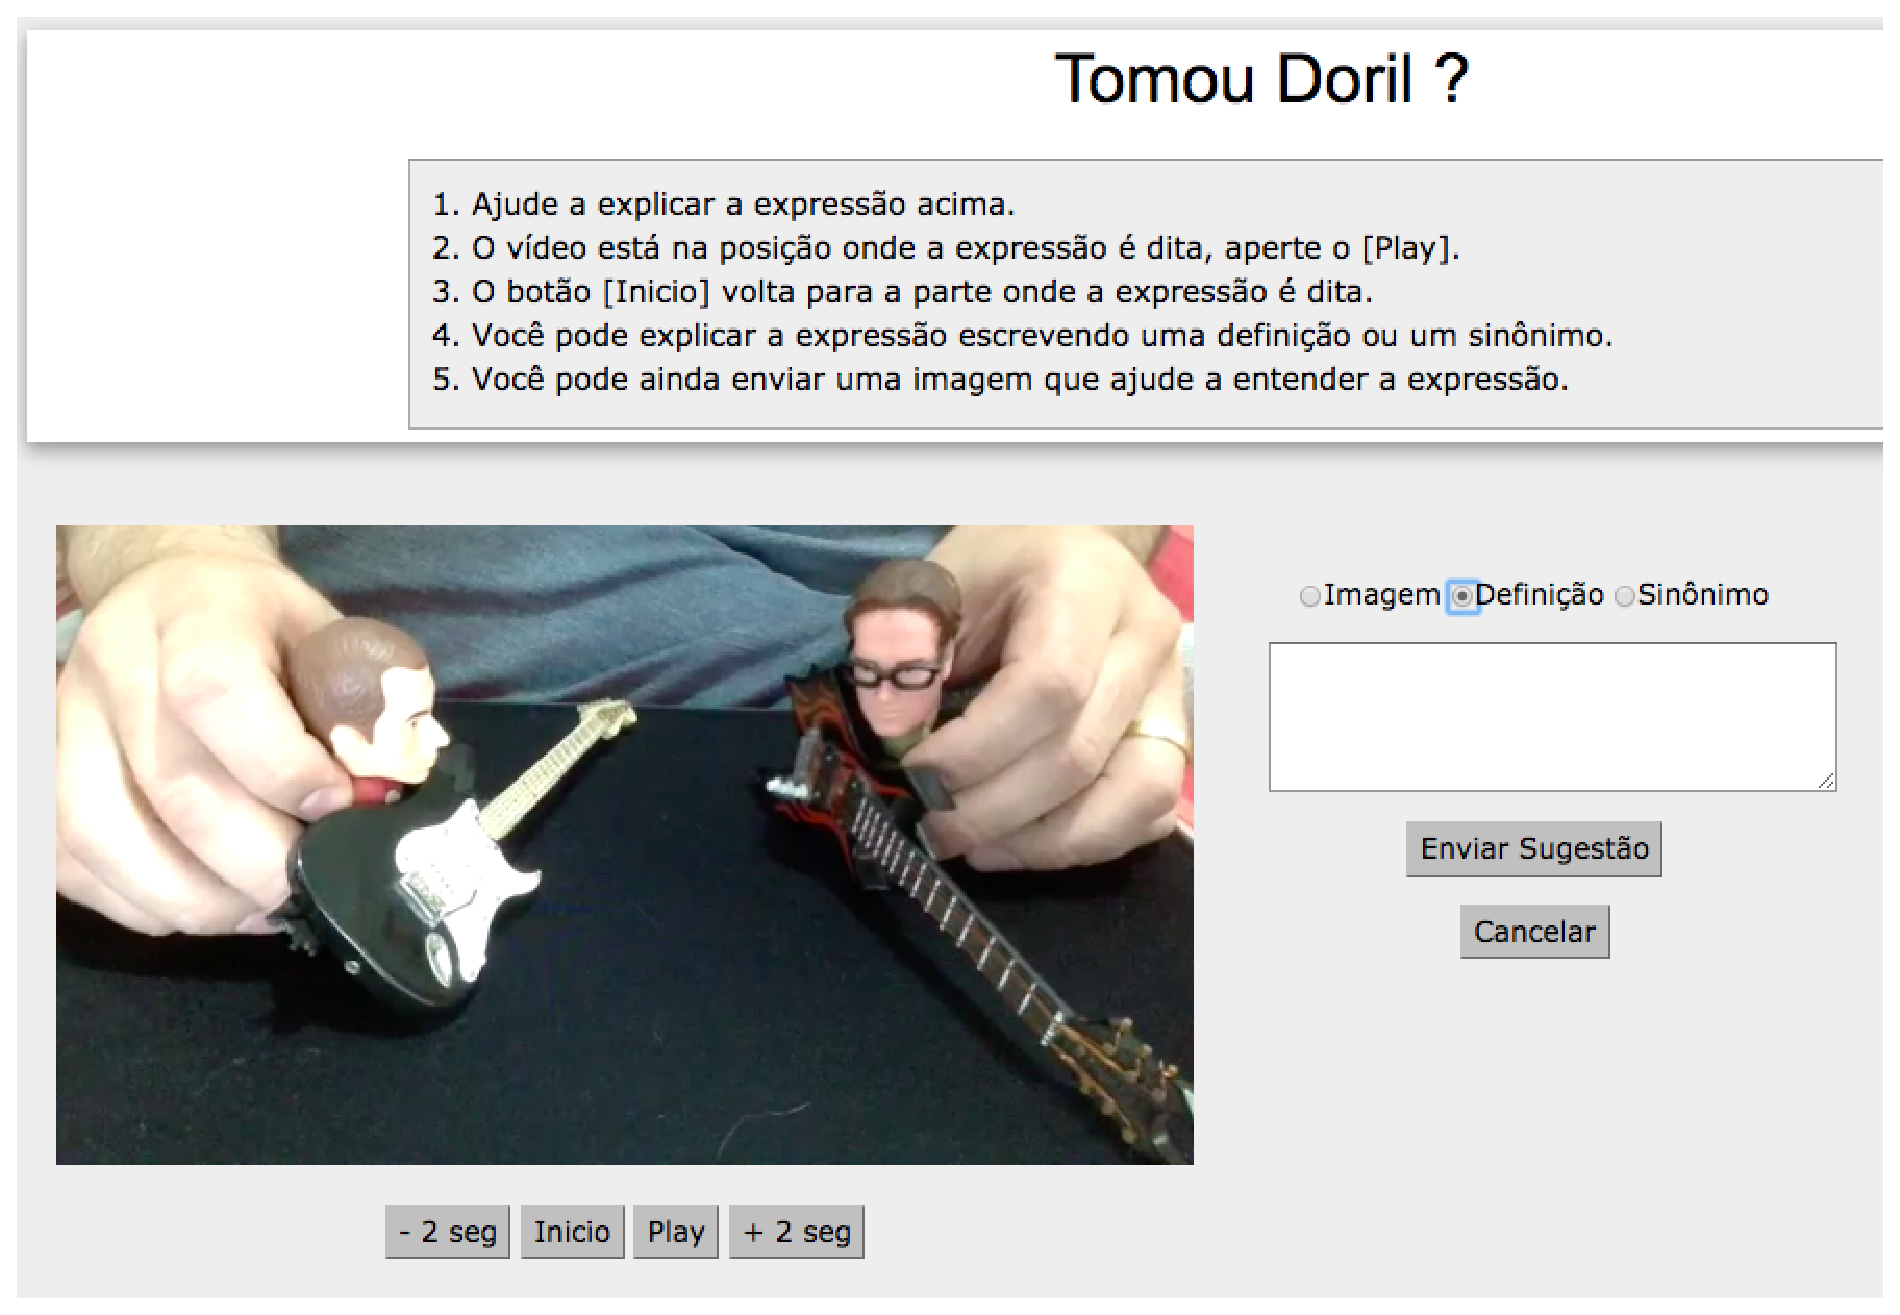
\includegraphics[scale=0.21] {figure/task2_c}}
	\caption{Annotation tool for task 2}
	\label{task2}
\end{figure}  

\item \textbf{Task 3:} The third annotation tool (Figure~\ref{task3}) presents to the collaborator a point of interest, also the different contents suggested to cover it. The contributor should navigate through the suggested content using the button bar on the contribution form and choose which one is most appropriate. %In addition, the collaborator can use the zoom button to better visualize the contents.

\begin{figure}[h]
	\centerline{\includegraphics[scale=0.14] {figure/task3_b}}
	\caption{Annotation tool for task 3}
	\label{task3}
\end{figure}  	
	
	
\item \textbf{Task 4:} The fourth annotation tool (Figure~\ref{task4}) shows the contributor the content chosen in task 3 to cover a point of interest, and asks to choose the best position in the scene to display by clicking on the desired position.

\begin{figure}[h]
	\centerline{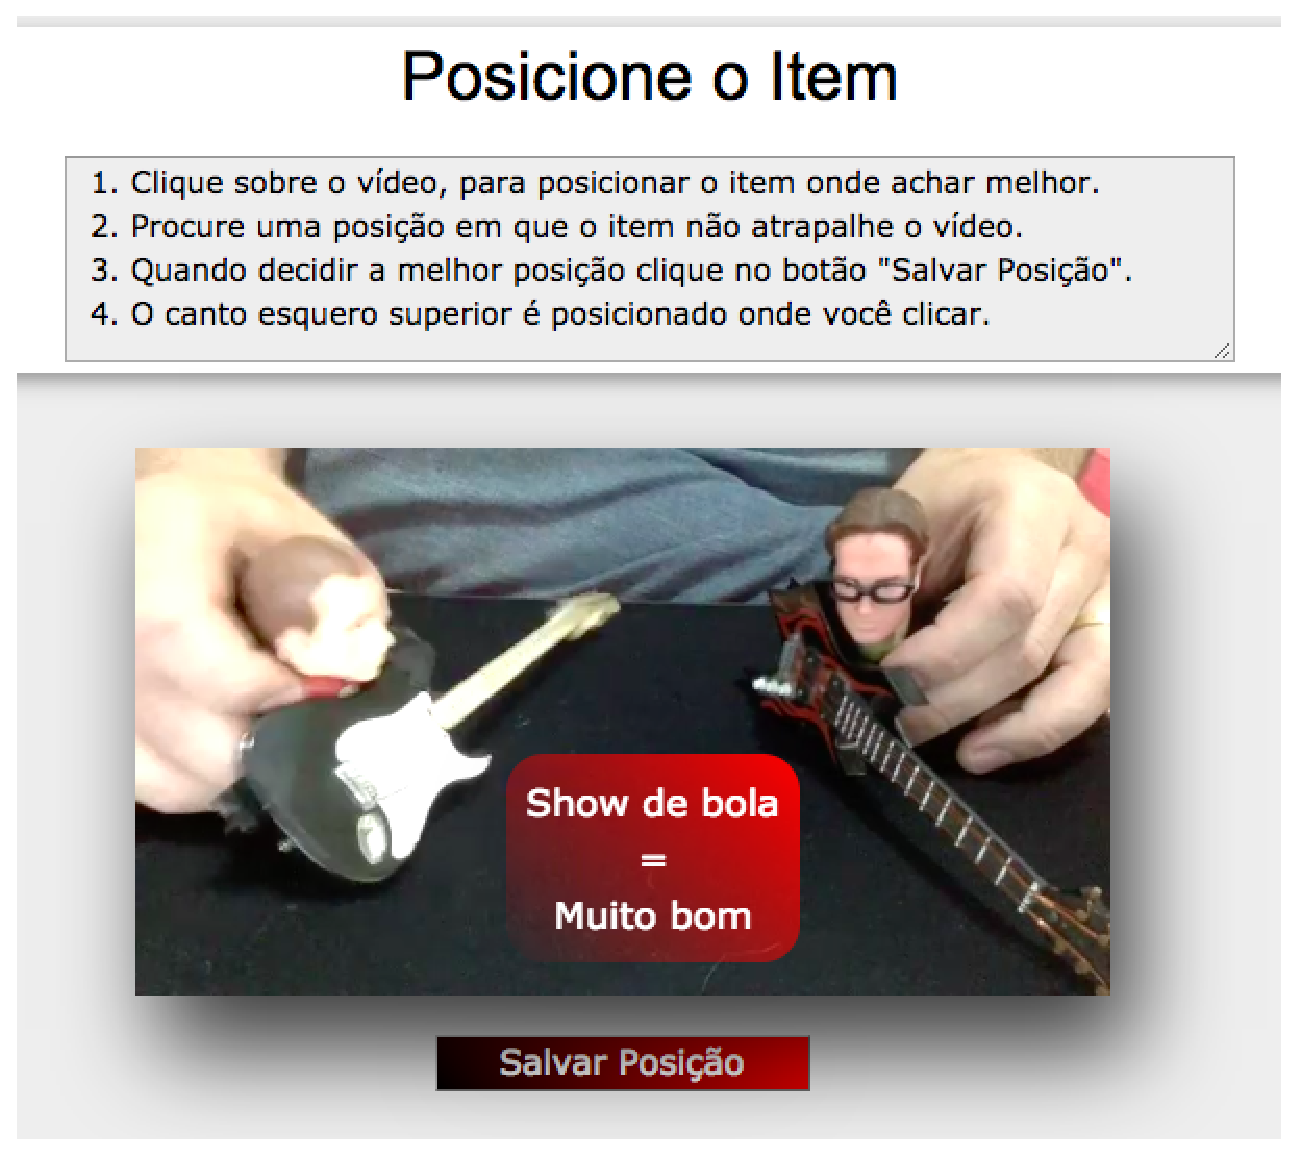
\includegraphics[scale=0.32] {figure/task4_c}}
	\caption{Annotation tool for task 4}
	\label{task4}
\end{figure}  	

\end{itemize}


\item \textbf{Write explanations about the microtask:} \linebreak 
The last activity of the preparation step in to write explanations about how to execute each annotation microtask. These explanations are very important because, in a crowdsourcing scenario, usually is not possible to instruct personally the workers about how to contribute.

For each annotation tool developed to this project, was written a sequence of instructions that explain how to use it. In all these tools, the instructions are presented on the top of the page, as illustrated on Figures~\ref{task1},~\ref{task2},~\ref{task3} and ~\ref{task4}.



\end{itemize}



\subsection{Step 2: Annotation}
	\begin{itemize}
		\item \textbf{Task 1 - Identify Points of Interest:} the first annotation microtask was supported by the tool represented in Figure~\ref{task1}, collecting identification for points of interest. In this task the contributor receive a segment of video that should be watched, and if was found any word, expression or information that require additional definitions or explanations, it should be marked as a point of interest.
		
		The segment of video sent to each user is chosen randomly according the criteria defined by the user. Two strategies was available to determine the segments: time length and semantic blocks. For this experiment was used semantic blocks, it means that for each video was previously defined start and stop times for segments of the video that should be presented as a semantic cell. This strategy demands an initial effort from the owner, but deliver to worker contextualized video segments. 
		
		Was collected 68 contributions and, after close the task and execute the aggregation method, they was merged into 37 different points of interest.

	
		\item \textbf{Task 2 - Suggesting Contribution Content:} the second task taken as input the aggregated result from the task 1, with 37 points of interest. In order to take advantage of the open call made for the task 1, was used the same URL redirecting the workers to the second annotation tool.
		
		The open call was reinforced by sharing  it on a social network, and it resulted in 308 contributions in 24 hours. After execute the second aggregation method, the 308 contributions was merged into 239 suggestions of content to cover the points of interest. These suggestions included plain text, images and hyperlinks.
		
	
	
		\item \textbf{Task 3 - Ranking Suggestions:} the third microtask aimed ranking the 239 suggested contents that resulted from the task 2. Was repeated the strategy of use the same URL for the new task, and reinforce the same open call.
		
		In this task was noticed a issue involving the suggestions associated to hyperlinks. Some of contributors related problems to visualize these suggestions such as "PAGE NOT FOUND" or "BLOCKED WEBSITE". Maybe because of this, most hyperlinks voted as most appropriated content point to Wikipedia or Youtube.
		
		The number of contributions collected in 24 hours was 255, and them were enough to determine the most appropriated content to all 37 points of interest.
	
		\item \textbf{Task 4 - Positioning Items:} by foreign affairs the fourth annotation microtask was performed about one week after the previous one. Because of this was opted for recruit contributors by a new open call. However, this open call was similar to the first one.
		
This microtask was the simplest task, and could be done in a few seconds. In 24 hours were collected 541 contributions that consisted in suggestions about in which position each item should be positioned over a video scene. These contributions were enough to determine the average position for all 37 points of interesting.
		
	\end{itemize}
		
\subsection{Step 3: Presentation}
With all annotations generated, the presentation system was able to use them to compose a presentation using both the original video and annotations.
	\begin{itemize}
		\item \textbf{Generating Outcome:} The annotations that represent the content that must be displayed to cover the interesting points have been manipulated in different ways according to their media types. The images were scaled according to the presentation area, the hyperlink was used to load previews for web pages, and the texts were formatted to be displayed correctly.
		
In addition, for each item, a second view was generated to be used in the zoom box, activated by the user to enlarge the items for a better visualization, as can be seen in the Figure~\ref{player_b}.
\begin{figure}[h]
	\centerline{\includegraphics[scale=0.2] {figure/player_b}}
	\caption{Extra content into the zoom box}
	\label{player_b}
\end{figure}  		
	
		\item \textbf{Presentation:} The presentation system can be seen on the Figure~\ref{player_a}. This system is capable of reproducing the original video synchronized with the extra content. When the user clicks on some extra content displayed in the video, the presentation is paused and a larger preview for the selected content is displayed in the zoom box as shown in the Figure~\ref{player_b}. 
		
This systems features navigation by extra-content instead the traditional timeline navigation, making available
 a button-bar with buttons to navigate among the extra contents.
		
 		
\begin{figure}[h]
	\centerline{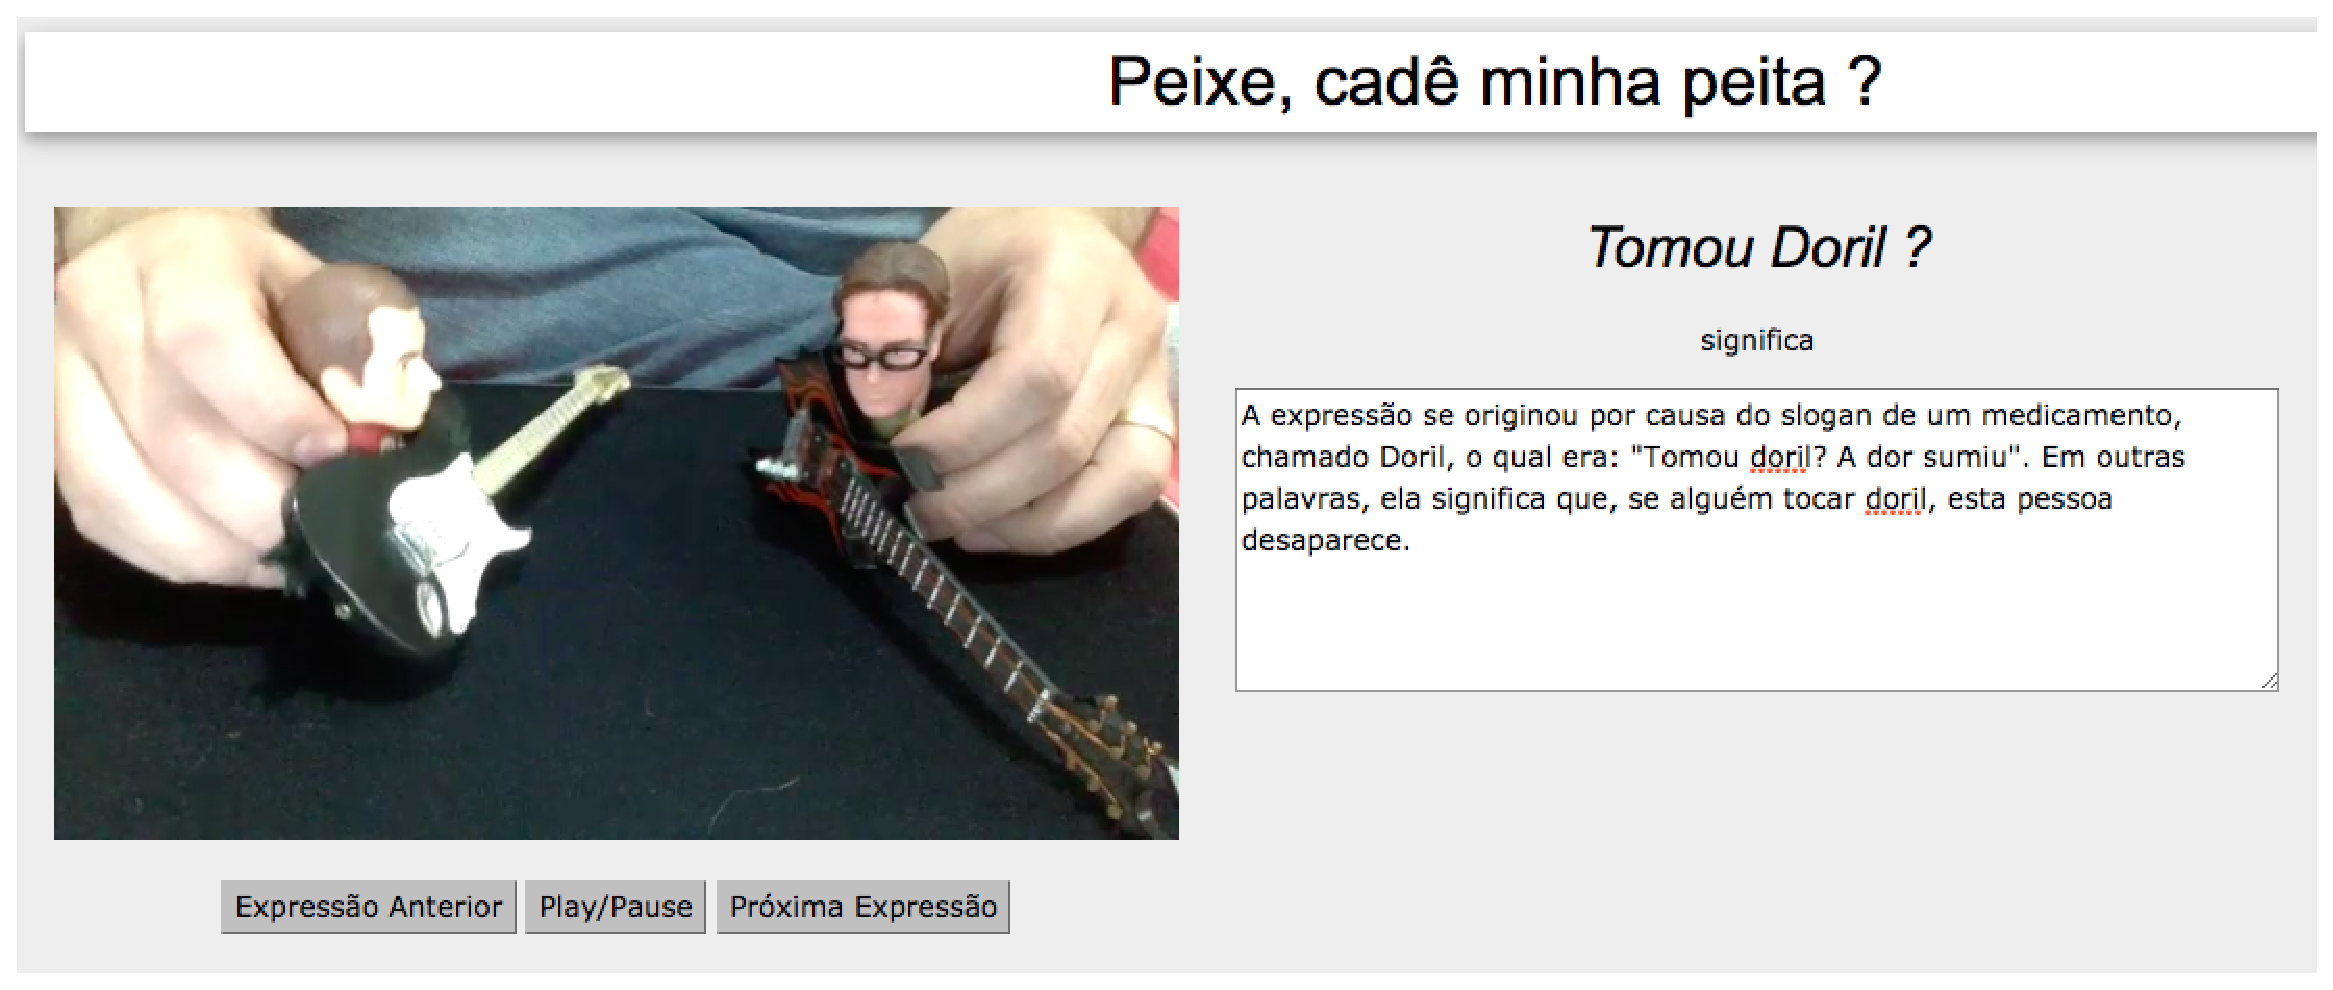
\includegraphics[scale=0.2] {figure/player_old}}
	\caption{Previous presentation system}
	\label{player_old}
\end{figure}  

The first version of the presentation system (Figure~\ref{player_old}) presented the extra content in a delimited area on the right side of the page. The reason for this is that Task 4 was not applied at the beginning, so the system did not have information on where to display the items on the video.

Fortunately, it was possible to perform the fourth microtask later and it was possible to create the new version of the presentation system (Figure~\ref{player_a}). In addition, this issue demonstrates that it is possible to reuse or improve an annotation system using this approach simply by adding new microtasks.

\begin{figure}[h]
	\centerline{\includegraphics[scale=0.35] {figure/player_a}}
	\caption{Presentation system}
	\label{player_a}
\end{figure} 

	
		
	\end{itemize}
	
	
	
	
	
	
	